% Options for packages loaded elsewhere
\PassOptionsToPackage{unicode}{hyperref}
\PassOptionsToPackage{hyphens}{url}
\PassOptionsToPackage{dvipsnames,svgnames,x11names}{xcolor}
%
\documentclass[
  title=normal,
  notoc,
  nobib,
  degree=mecinf]{mnye}
\usepackage{amsmath,amssymb}
\usepackage{lmodern}
\usepackage{iftex}
\ifPDFTeX
  \usepackage[T1]{fontenc}
  \usepackage[utf8]{inputenc}
  \usepackage{textcomp} % provide euro and other symbols
\else % if luatex or xetex
  \usepackage{unicode-math}
  \defaultfontfeatures{Scale=MatchLowercase}
  \defaultfontfeatures[\rmfamily]{Ligatures=TeX,Scale=1}
\fi
% Use upquote if available, for straight quotes in verbatim environments
\IfFileExists{upquote.sty}{\usepackage{upquote}}{}
\IfFileExists{microtype.sty}{% use microtype if available
  \usepackage[]{microtype}
  \UseMicrotypeSet[protrusion]{basicmath} % disable protrusion for tt fonts
}{}
\makeatletter
\@ifundefined{KOMAClassName}{% if non-KOMA class
  \IfFileExists{parskip.sty}{%
    \usepackage{parskip}
  }{% else
    \setlength{\parindent}{0pt}
    \setlength{\parskip}{6pt plus 2pt minus 1pt}}
}{% if KOMA class
  \KOMAoptions{parskip=half}}
\makeatother
\usepackage{xcolor}
\IfFileExists{xurl.sty}{\usepackage{xurl}}{} % add URL line breaks if available
\IfFileExists{bookmark.sty}{\usepackage{bookmark}}{\usepackage{hyperref}}
\hypersetup{
  pdftitle={Inferencias sobre una media},
  pdfauthor={Eva María Mazcuñán Navarro},
  colorlinks=true,
  linkcolor={Maroon},
  filecolor={Maroon},
  citecolor={Blue},
  urlcolor={Blue},
  pdfcreator={LaTeX via pandoc}}
\urlstyle{same} % disable monospaced font for URLs
\usepackage{color}
\usepackage{fancyvrb}
\newcommand{\VerbBar}{|}
\newcommand{\VERB}{\Verb[commandchars=\\\{\}]}
\DefineVerbatimEnvironment{Highlighting}{Verbatim}{commandchars=\\\{\}}
% Add ',fontsize=\small' for more characters per line
\usepackage{framed}
\definecolor{shadecolor}{RGB}{248,248,248}
\newenvironment{Shaded}{\begin{snugshade}}{\end{snugshade}}
\newcommand{\AlertTok}[1]{\textcolor[rgb]{0.94,0.16,0.16}{#1}}
\newcommand{\AnnotationTok}[1]{\textcolor[rgb]{0.56,0.35,0.01}{\textbf{\textit{#1}}}}
\newcommand{\AttributeTok}[1]{\textcolor[rgb]{0.77,0.63,0.00}{#1}}
\newcommand{\BaseNTok}[1]{\textcolor[rgb]{0.00,0.00,0.81}{#1}}
\newcommand{\BuiltInTok}[1]{#1}
\newcommand{\CharTok}[1]{\textcolor[rgb]{0.31,0.60,0.02}{#1}}
\newcommand{\CommentTok}[1]{\textcolor[rgb]{0.56,0.35,0.01}{\textit{#1}}}
\newcommand{\CommentVarTok}[1]{\textcolor[rgb]{0.56,0.35,0.01}{\textbf{\textit{#1}}}}
\newcommand{\ConstantTok}[1]{\textcolor[rgb]{0.00,0.00,0.00}{#1}}
\newcommand{\ControlFlowTok}[1]{\textcolor[rgb]{0.13,0.29,0.53}{\textbf{#1}}}
\newcommand{\DataTypeTok}[1]{\textcolor[rgb]{0.13,0.29,0.53}{#1}}
\newcommand{\DecValTok}[1]{\textcolor[rgb]{0.00,0.00,0.81}{#1}}
\newcommand{\DocumentationTok}[1]{\textcolor[rgb]{0.56,0.35,0.01}{\textbf{\textit{#1}}}}
\newcommand{\ErrorTok}[1]{\textcolor[rgb]{0.64,0.00,0.00}{\textbf{#1}}}
\newcommand{\ExtensionTok}[1]{#1}
\newcommand{\FloatTok}[1]{\textcolor[rgb]{0.00,0.00,0.81}{#1}}
\newcommand{\FunctionTok}[1]{\textcolor[rgb]{0.00,0.00,0.00}{#1}}
\newcommand{\ImportTok}[1]{#1}
\newcommand{\InformationTok}[1]{\textcolor[rgb]{0.56,0.35,0.01}{\textbf{\textit{#1}}}}
\newcommand{\KeywordTok}[1]{\textcolor[rgb]{0.13,0.29,0.53}{\textbf{#1}}}
\newcommand{\NormalTok}[1]{#1}
\newcommand{\OperatorTok}[1]{\textcolor[rgb]{0.81,0.36,0.00}{\textbf{#1}}}
\newcommand{\OtherTok}[1]{\textcolor[rgb]{0.56,0.35,0.01}{#1}}
\newcommand{\PreprocessorTok}[1]{\textcolor[rgb]{0.56,0.35,0.01}{\textit{#1}}}
\newcommand{\RegionMarkerTok}[1]{#1}
\newcommand{\SpecialCharTok}[1]{\textcolor[rgb]{0.00,0.00,0.00}{#1}}
\newcommand{\SpecialStringTok}[1]{\textcolor[rgb]{0.31,0.60,0.02}{#1}}
\newcommand{\StringTok}[1]{\textcolor[rgb]{0.31,0.60,0.02}{#1}}
\newcommand{\VariableTok}[1]{\textcolor[rgb]{0.00,0.00,0.00}{#1}}
\newcommand{\VerbatimStringTok}[1]{\textcolor[rgb]{0.31,0.60,0.02}{#1}}
\newcommand{\WarningTok}[1]{\textcolor[rgb]{0.56,0.35,0.01}{\textbf{\textit{#1}}}}
\usepackage{longtable,booktabs,array}
\usepackage{calc} % for calculating minipage widths
% Correct order of tables after \paragraph or \subparagraph
\usepackage{etoolbox}
\makeatletter
\patchcmd\longtable{\par}{\if@noskipsec\mbox{}\fi\par}{}{}
\makeatother
% Allow footnotes in longtable head/foot
\IfFileExists{footnotehyper.sty}{\usepackage{footnotehyper}}{\usepackage{footnote}}
\makesavenoteenv{longtable}
\usepackage{graphicx}
\makeatletter
\def\maxwidth{\ifdim\Gin@nat@width>\linewidth\linewidth\else\Gin@nat@width\fi}
\def\maxheight{\ifdim\Gin@nat@height>\textheight\textheight\else\Gin@nat@height\fi}
\makeatother
% Scale images if necessary, so that they will not overflow the page
% margins by default, and it is still possible to overwrite the defaults
% using explicit options in \includegraphics[width, height, ...]{}
\setkeys{Gin}{width=\maxwidth,height=\maxheight,keepaspectratio}
% Set default figure placement to htbp
\makeatletter
\def\fps@figure{htbp}
\makeatother
\setlength{\emergencystretch}{3em} % prevent overfull lines
\providecommand{\tightlist}{%
  \setlength{\itemsep}{0pt}\setlength{\parskip}{0pt}}
\setcounter{secnumdepth}{5}
\usepackage{ehyperref}
\colorlet{etoccolor}{greenlink}
% This file is created the first time epdf_document is invoked
% but will not be overwriten afterwards.
%
% Preamble

\usepackage{ebox}
\usepackage{enotation}
\usepackage{fontawesome}

% https://stackoverflow.com/questions/63222203/rmarkdown-wrap-code-in-chunks-but-keep-breaks-after-pipe
\usepackage{fvextra}
\DefineVerbatimEnvironment{Highlighting}{Verbatim}{
    breaksymbolleft={},
    showspaces = false,
    showtabs = false,
    breaklines,
    commandchars=\\\{\}
}

\pgfplotsset{compat=1.18}
\degree{Grado en Ingeniería Informática/Mecánica}
\term{2021-2022}
\ifLuaTeX
  \usepackage{selnolig}  % disable illegal ligatures
\fi
\usepackage[]{biblatex}
\addbibresource{book.bib}
\addbibresource{packages.bib}

\title{Inferencias sobre una media}
\author{Eva María Mazcuñán Navarro}
\date{}

\begin{document}
\maketitle

% This file is created the first time epdf_document is invoked
% but will not be overwriten afterwards.
%
% Before Body

{
\hypersetup{linkcolor=etoccolor}
\setcounter{tocdepth}{2}
\tableofcontents
}
\hypertarget{section}{%
\section*{}\label{section}}

\hypertarget{intro}{%
\section*{Introducción}\label{intro}}
\addcontentsline{toc}{section}{Introducción}

En el tema \textbf{Inferencia Estadística} se estudiaron los fundamentos de las principales técnicas de inferencia estadística: los contrastes de hipótesis y los intervalos de confianza. Se presentaron los nuevos conceptos partiendo del caso particular de un problema de inferencia para una \textbf{proporción}.

En esta práctica se aplicarán las mencionadas técnicas para realizar inferencias sobre un nuevo parámetro: la \textbf{media} de una variable continua.

\hypertarget{prerequisites}{%
\subsection*{Requisitos previos}\label{prerequisites}}
\addcontentsline{toc}{subsection}{Requisitos previos}

Antes de comenzar esta práctica, necesitas:

\begin{itemize}
\item
  Tener \textsf{R} y \textsf{RStudio} instalados en tu equipo (ver \href{https://emazcunan.github.io/install-r-rstudio/}{Instalación de R y RStudio}).
\item
  Haber estudiado la práctica \href{https://emazcunan.github.io/basics-r-rstudio/}{Primeros pasos con R y RStudio}.
\item
  Haber estudiado el tema \textbf{Inferencia Estadística}.
\end{itemize}

\hypertarget{workflow}{%
\subsection*{Flujo de trabajo}\label{workflow}}
\addcontentsline{toc}{subsection}{Flujo de trabajo}

Documenta lo que vayas aprendiendo conforme leas la práctica usando un documento R Markdown. Puedes utilizar \href{https://drive.google.com/uc?id=1t9pjP_1Kjo8wgtav_I6hPHXxb5BqTIrc\&export=download}{esta plantilla}.

Se recomienda guardar el archivo R Markdown en una carpeta propia. En dicha carpeta se creará el archivo \textsf{HTML} resultante de la compilación y después añadiremos los archivos con los datos que usaremos a lo largo de la práctica.

Recuerda que para crear encabezados se utiliza la sintaxis \texttt{\#} (nivel 1), \texttt{\#\#} (nivel 2), \ldots; y que los bloques de código se crean con el atajo \texttt{Ctrl\ +\ Alt\ +\ I}.

Respecto al seccionado del documento, lo más práctico es que imites la estructura de este guión de prácticas.

\hypertarget{packages}{%
\section{Paquetes}\label{packages}}

Como en las prácticas anteriores, cargamos el paquete \texttt{tidyverse} para que estén disponibles las funciones que utilizaremos:

\begin{Shaded}
\begin{Highlighting}[]
\FunctionTok{library}\NormalTok{(tidyverse)}
\end{Highlighting}
\end{Shaded}

\hypertarget{problem}{%
\section{Planteamiento del problema}\label{problem}}

\begin{ebox}{}
Una empresa de domótica comercializa un modelo de mandos a distancia para la apertura de puertas de garaje.

Estamos interesados en investigar el radio de alcance medio de este modelo de mandos, siendo el radio de alcance de un mando la distancia máxima medida en metros a la que el mando consigue abrir la puerta.

La empresa afirma que el radio de alcance medio de sus mandos es superior a \(50\) metros. Se tomó una muestra \(100\) mandos y se midió su radio de alcance, con el objetivo de contrastar si los datos recogidos resultan compatibles con la afirmación de la empresa.

\end{ebox}

Consideremos la variable aleatoria

\begin{center}
\(X =\) radio de alcance de un mando, en metros.

\end{center}

Nuestro objetivo es investigar el valor del parámetro
\[
\mu = E(X),
\]
la media o valor esperado de la variable \(X\).

En el archivo enlazado a continuación se registran los radios de alcance de los \(100\) mandos analizados: \href{https://drive.google.com/uc?id=1dDOdobanG-_ZTTh0mx1R6KRSrnvtD8gL\&export=download}{mandos.csv}. En el resto de la práctica se asume que el archivo \texttt{mandos.csv} está ubicado en un directorio de nombre \texttt{data} dentro del directorio en el que se encuentre el archivo \texttt{.Rmd} con el código.

En esta práctica exploraremos qué conclusiones o inferencias podemos realizar sobre el parámetro desconocido \(\mu\), a partir de las \(100\) mediciones realizadas.

\begin{center}\rule{0.5\linewidth}{0.5pt}\end{center}

Importamos los datos del problema con la instrucción

\begin{Shaded}
\begin{Highlighting}[]
\NormalTok{mandos }\OtherTok{\textless{}{-}} \FunctionTok{read\_csv}\NormalTok{(}\StringTok{"data/mandos.csv"}\NormalTok{)}
\end{Highlighting}
\end{Shaded}

que creará la hoja de datos \texttt{mandos} con los contenidos del archivo \texttt{mandos.csv}.

Al visualizar el objeto \texttt{mandos} recién creado (desde la pestaña Environment) verás que tiene una única variable, de nombre \texttt{alcance}, en la que se registra el radio de alcance medido para cada uno de los \(100\) mandos analizados.

\hypertarget{descriptive}{%
\section{Estadística descriptiva}\label{descriptive}}

Como punto de partida de nuestro estudio, realizaremos un análisis exploratorio de nuestros datos, incluyendo:

\begin{itemize}
\item
  El cálculo de la media muestral \(\bar x\), como estimación puntual de la media poblacional \(\mu\).
\item
  El cálculo de otras medidas descriptivas, tales como la desviación típica muestral y los cuartiles.
\item
  La representación gráfica de los datos mediante un histograma y un diagrama de caja y bigotes.
\end{itemize}

\hypertarget{mean}{%
\subsection{Media muestral}\label{mean}}

Una forma natural de estimar el valor de la media teórica \(\mu\) es calcular la media aritmética o promedio del radio de alcance de los \(100\) mandos analizados, que calculamos con la instrucción:

\begin{Shaded}
\begin{Highlighting}[]
\FunctionTok{mean}\NormalTok{(mandos}\SpecialCharTok{$}\NormalTok{alcance)}
\end{Highlighting}
\end{Shaded}

\begin{Shaded}
\begin{Highlighting}[]
\NormalTok{\#\# [1] 48.8852}
\end{Highlighting}
\end{Shaded}

La expresión \VERB|\NormalTok{mandos}\SpecialCharTok{$}\NormalTok{alcance}| extrae la variable \texttt{alcance} de la hoja de datos \texttt{mandos} y la función \VERB|\FunctionTok{mean}\NormalTok{()}| calcula el promedio del vector resultante.

En general, dadas \(n\) observaciones \(x_1\), \(x_2\), \(\dots\), \(x_n\) de una variable aleatoria continua \(X\) la cantidad
\[
    \bar{x} = \frac{x_1 + x_2 + \dots + x_n}{n}
\]
se llama \textbf{media muestral} y proporciona una estimación puntual de la \textbf{media poblacional} \(\mu = E(X)\).

La media muestral \(\overline{x} = 48.8852\) de nuestros datos nos proporciona una estimación de \(\mu\), pero hay que tener claro que el verdadero valor de \(\mu\) sigue siendo desconocido:

\begin{itemize}
\tightlist
\item
  El verdadero valor de \(\mu\) es la media o valor esperado de la variable aleatoria \(X\). Según hemos estudiado en la teoría, identificamos \(\mu\) con el valor medio teórico del radio de alcance de todos los mandos fabricados por la empresa, con el valor límite al que tendería el alcance promedio observado para \(n\) mandos cuando \(n\) tiende a infinito.\\
\item
  Por su parte, el valor \(\overline{x} = 48.8852\) es tan sólo el radio de alcance promedio de los \(n=100\) mandos que hemos observado.
\end{itemize}

Podría ser que \(\mu=53\), en cuyo caso los \(100\) mandos observados tendrían un radio de alcance promedio inferior a la media teórica \(\mu\). Y de la misma forma podría ser \(\mu=45\), y que hayamos observado por azar \(100\) mandos con radio de alcance promedio superior a la media teórica \(\mu\).

\hypertarget{sd}{%
\subsection{Varianza muestral y desviación típica muestral}\label{sd}}

Dadas \(n\) observaciones \(x_1\), \(x_2\), \(\dots\), \(x_n\) de una variable aleatoria continua \(X\), su \textbf{varianza muestral} se define como
\[
    s^2 = \frac{(x_1-\bar{x})^2 + (x_2-\bar{x})^2 + \dots + (x_n-\bar{x})^2}{n-1}
\]
y proporciona una estimación puntual de la \textbf{varianza poblacional} \(\sigma^2 = Var(X)\).

Notar que se divide por \(n-1\) y no por \(n\), por razones técnicas para las que por ahora podemos dar la siguiente explicación informal: En la fórmula de \(s^2\) estamos utilizando la media muestral \(\bar x\) de las \(n\) observaciones \(x_i\), que representan una muestra de la población con media \(\mu\). Y conociendo la media muestral, solo \(n-1\) de los \(n\) valores \(x_i\) pueden variar libremente. Se demuestra que si para calcular \(s^2\) dividiéramos por \(n\), en lugar de \(n-1\), el valor obtenido tiende a subestimar el verdadero valor de la varianza poblacional \(\sigma^2\).

La \textbf{desviación típica muestral} es la raíz cuadrada de la varianza muestral:
\[s=\sqrt{s^2}.\]

Para calcular la desviación típica muestral de nuestros datos usamos la función \VERB|\FunctionTok{sd}\NormalTok{()}|:

\begin{Shaded}
\begin{Highlighting}[]
\FunctionTok{sd}\NormalTok{(mandos}\SpecialCharTok{$}\NormalTok{alcance)}
\end{Highlighting}
\end{Shaded}

\begin{Shaded}
\begin{Highlighting}[]
\NormalTok{\#\# [1] 7.554216}
\end{Highlighting}
\end{Shaded}

\hypertarget{quantiles}{%
\subsection{Cuantiles}\label{quantiles}}

Dadas \(n\) observaciones \(x_1\), \(x_2\), \(\dots\), \(x_n\) de una variable aleatoria continua \(X\) y un valor \(\alpha\) entre \(0\) y \(1\), se define el \textbf{cuantil de orden \(\alpha\)} de dichas observaciones como el valor que, en la secuencia ordenada de valores de menor a mayor, queda situado de forma que divide la muestra en dos partes, dejando por debajo una fracción o proporción \(\alpha\) de los valores.

Por ejemplo, el cuantil de orden \(0.1\), posicionado en la secuencia ordenada de valores, dejaría al \(10\%\) de las observaciones por debajo y al \(90\%\) restante por arriba.

Como casos particulares de cuantiles tenemos los \textbf{cuartiles}:

\begin{itemize}
\item
  El \textbf{primer cuartil} es el cuantil \(0.25\), esto es, el valor que deja por debajo el \(25\%\) de los datos (y por arriba el \(75\%\) restante).
\item
  El \textbf{segundo cuartil} o \textbf{mediana} es el cuantil \(0.25\), o lo que es lo mismo, el valor que deja por debajo el \(50\%\) de los datos (y por arriba el otro \(50\%\)).
\item
  Y el \textbf{tercer cuartil} es el cuantil \(0.75\), es decir el valor que deja por debajo el \(75\%\) de los datos (y por arriba el \(25\%\) restante).
\end{itemize}

Calculamos el primer cuartil, la mediana, y el tercer cuartil de nuestra muestra con la siguiente instrucción:

\begin{Shaded}
\begin{Highlighting}[]
\FunctionTok{quantile}\NormalTok{(mandos}\SpecialCharTok{$}\NormalTok{alcance, }\AttributeTok{probs =} \FunctionTok{c}\NormalTok{(}\FloatTok{0.25}\NormalTok{, }\FloatTok{0.5}\NormalTok{, }\FloatTok{0.75}\NormalTok{))}
\end{Highlighting}
\end{Shaded}

\begin{Shaded}
\begin{Highlighting}[]
\NormalTok{\#\#    25\%    50\%    75\% }
\NormalTok{\#\# 44.545 49.520 54.660}
\end{Highlighting}
\end{Shaded}

El primer cuartil resulta ser \(44.545\), la mediana \(49.52\), y el tercer cuartil \(54.66\). Veamos por ejemplo cómo se ha obtenido el valor \(49.52\) para la mediana, que deja el \(50\%\) de los datos por debajo y la otra mitad por arriba. En primer lugar ordenamos nuestros datos, de menor a mayor, con la orden:

\begin{Shaded}
\begin{Highlighting}[]
\FunctionTok{sort}\NormalTok{(mandos}\SpecialCharTok{$}\NormalTok{alcance)}
\end{Highlighting}
\end{Shaded}

\begin{Shaded}
\begin{Highlighting}[]
\NormalTok{\#\#   [1] 28.26 29.78 35.32 36.08 36.39 36.74 36.82 37.01 37.13 37.24 38.65 39.07}
\NormalTok{\#\#  [13] 39.88 40.85 40.85 41.10 41.25 41.37 42.36 42.60 43.15 43.26 43.38 44.04}
\NormalTok{\#\#  [25] 44.47 44.57 44.58 44.67 44.82 45.19 45.23 45.37 45.39 45.68 45.76 45.90}
\NormalTok{\#\#  [37] 45.99 46.04 46.07 46.50 46.56 46.99 47.12 48.06 48.14 48.32 48.79 48.88}
\NormalTok{\#\#  [49] 49.35 49.36 49.68 49.94 49.96 49.97 50.12 50.32 50.52 50.53 50.56 50.58}
\NormalTok{\#\#  [61] 50.76 50.83 51.04 51.30 51.74 52.19 52.37 53.50 53.58 53.94 54.22 54.31}
\NormalTok{\#\#  [73] 54.42 54.59 54.59 54.87 55.05 55.06 55.23 55.39 55.52 55.58 56.12 56.68}
\NormalTok{\#\#  [85] 56.79 56.90 56.98 56.99 57.01 57.35 57.59 58.78 58.96 60.17 60.18 60.57}
\NormalTok{\#\#  [97] 60.85 62.72 65.00 66.24}
\end{Highlighting}
\end{Shaded}

En la salida del comando anterior verás que:

\begin{itemize}
\item
  El dato que ocupa la posición \(50\) en la secuencia de valores ordenados, es \(49.36\) (recuerda que tienes que fijarte en los números entre corchetes al principio de cada línea de la salida para saber qué posición ocupa cada dato). Este valor deja \(49\) valores por debajo, y \(50\) por arriba.
\item
  Y el dato que ocupa la posición \(51\), es \(49.68\). Deja \(50\) valores por debajo y \(49\) por arriba.
\end{itemize}

Así, ni \(49.36\) (posición \(50\)), ni \(49.68\) (posición \(51\)), dejan justo la mitad de los datos por debajo y la otra mitad por arriba.
La posición ideal para la mediana sería la posición \(50.5\). Por esta razón, el cálculo que hace \textsf{R} para obtener la mediana es
\[
\frac{49.36+49.68}{2}=49.52,
\]
la media aritmética entre el dato de la posición \(50\) y el de la posición \(51\).

\hypertarget{summarize}{%
\subsection{\texorpdfstring{La función \texttt{summarize()}}{La función summarize()}}\label{summarize}}

La siguiente instrucción utiliza la función \VERB|\FunctionTok{summarize}\NormalTok{()}| para obtener todas las medidas descriptivas que se han calculado de forma individual en los apartados anteriores:

\begin{Shaded}
\begin{Highlighting}[]
\FunctionTok{summarize}\NormalTok{(}
  \AttributeTok{.data =}\NormalTok{ mandos,}
  \StringTok{"Media"} \OtherTok{=} \FunctionTok{mean}\NormalTok{(alcance),}
  \StringTok{"Desv. estandar"} \OtherTok{=} \FunctionTok{sd}\NormalTok{(alcance),}
  \StringTok{"1er cuartil"} \OtherTok{=} \FunctionTok{quantile}\NormalTok{(alcance, }\FloatTok{0.25}\NormalTok{),}
  \StringTok{"Mediana"} \OtherTok{=} \FunctionTok{quantile}\NormalTok{(alcance, }\FloatTok{0.5}\NormalTok{),}
  \StringTok{"3er cuartil"} \OtherTok{=} \FunctionTok{quantile}\NormalTok{(alcance, }\FloatTok{0.75}\NormalTok{)}
\NormalTok{)}
\end{Highlighting}
\end{Shaded}

\begin{Shaded}
\begin{Highlighting}[]
\NormalTok{\#\# \# A tibble: 1 x 5}
\NormalTok{\#\#   Media \textasciigrave{}Desv. estandar\textasciigrave{} \textasciigrave{}1er cuartil\textasciigrave{} Mediana \textasciigrave{}3er cuartil\textasciigrave{}}
\NormalTok{\#\#   \textless{}dbl\textgreater{}            \textless{}dbl\textgreater{}         \textless{}dbl\textgreater{}   \textless{}dbl\textgreater{}         \textless{}dbl\textgreater{}}
\NormalTok{\#\# 1  48.9             7.55          44.5    49.5          54.7}
\end{Highlighting}
\end{Shaded}

El valor \texttt{mandos} del primer argumento \texttt{.data} indica la hoja de datos en la que se encuentran las variables de interés. En el resto de argumentos se especifican los estadísticos para resumir los datos que se quieren calcular. Por ejemplo, el argumento \VERB|\StringTok{"Media"} \OtherTok{=} \FunctionTok{mean}\NormalTok{(alcance)}| en nuestro ejemplo solicita calcular la media de la variable \texttt{alcance} y le asigna el nombre \texttt{"Media"}. Las variables de la hoja de datos pueden usarse escribiendo solo su nombre (escribiendo solo \texttt{alcance} en lugar de \VERB|\NormalTok{mandos}\SpecialCharTok{$}\NormalTok{alcance}|). La salida se organiza como una nueva hoja de datos, con una columna con el valor de cada estadístico pedido, rotulada con el nombre que se haya indicado.

\hypertarget{histogram}{%
\subsection{Histograma}\label{histogram}}

Los \textbf{histogramas} son uno de los gráficos más comunes para representar una variable continua. Para obtener un histograma del alcance de los mandos en nuestra muestra utilizamos la función \VERB|\FunctionTok{geom\_histogram}\NormalTok{()}|:

\begin{Shaded}
\begin{Highlighting}[]
\FunctionTok{ggplot}\NormalTok{(}
  \AttributeTok{data =}\NormalTok{ mandos,}
  \AttributeTok{mapping =} \FunctionTok{aes}\NormalTok{(}\AttributeTok{x =}\NormalTok{ alcance)}
\NormalTok{) }\SpecialCharTok{+}
  \FunctionTok{geom\_histogram}\NormalTok{()}
\end{Highlighting}
\end{Shaded}

\begin{center}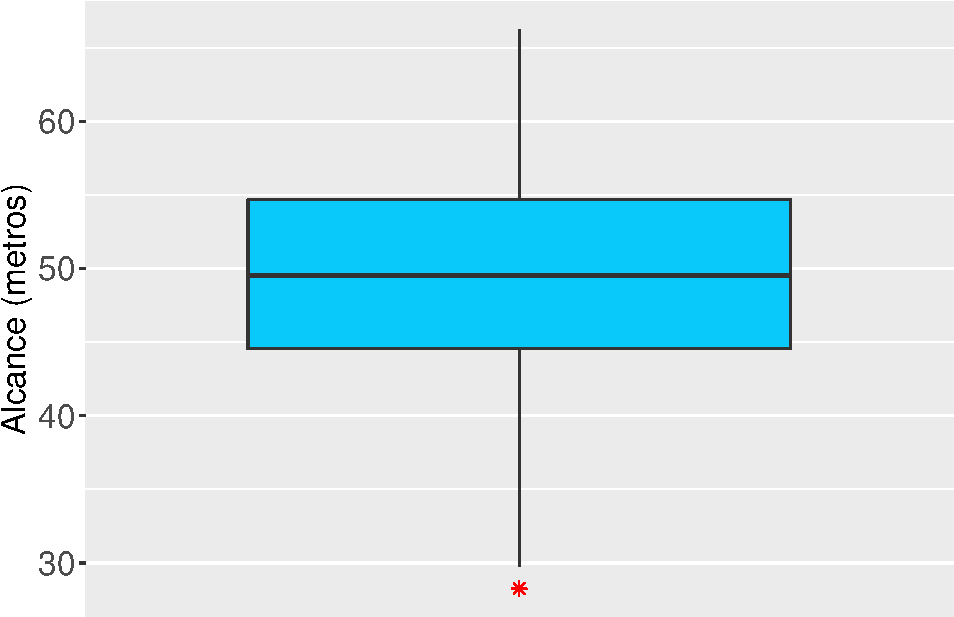
\includegraphics[width=0.8\linewidth]{one_mean_files/figure-latex/unnamed-chunk-24-1} \end{center}

Con el siguiente código se mejora el histograma anterior usando intervalos de anchura \(5\) (\VERB|\NormalTok{binwidth }\OtherTok{=} \DecValTok{5}|), personalizando el color de las barras y añadiendo rótulos a los ejes:

\begin{Shaded}
\begin{Highlighting}[]
\FunctionTok{ggplot}\NormalTok{(}
  \AttributeTok{data =}\NormalTok{ mandos,}
  \AttributeTok{mapping =} \FunctionTok{aes}\NormalTok{(}\AttributeTok{x =}\NormalTok{ alcance)}
\NormalTok{) }\SpecialCharTok{+}
  \FunctionTok{geom\_histogram}\NormalTok{(}
    \AttributeTok{binwidth =} \DecValTok{5}\NormalTok{,}
    \AttributeTok{color =} \StringTok{"black"}\NormalTok{,}
    \AttributeTok{fill =} \StringTok{"\#F98D08"}
\NormalTok{  ) }\SpecialCharTok{+}
  \FunctionTok{labs}\NormalTok{(}
    \AttributeTok{x =} \StringTok{"Alcance (metros)"}\NormalTok{,}
    \AttributeTok{y =} \StringTok{"Recuento"}
\NormalTok{  )}
\end{Highlighting}
\end{Shaded}

\begin{center}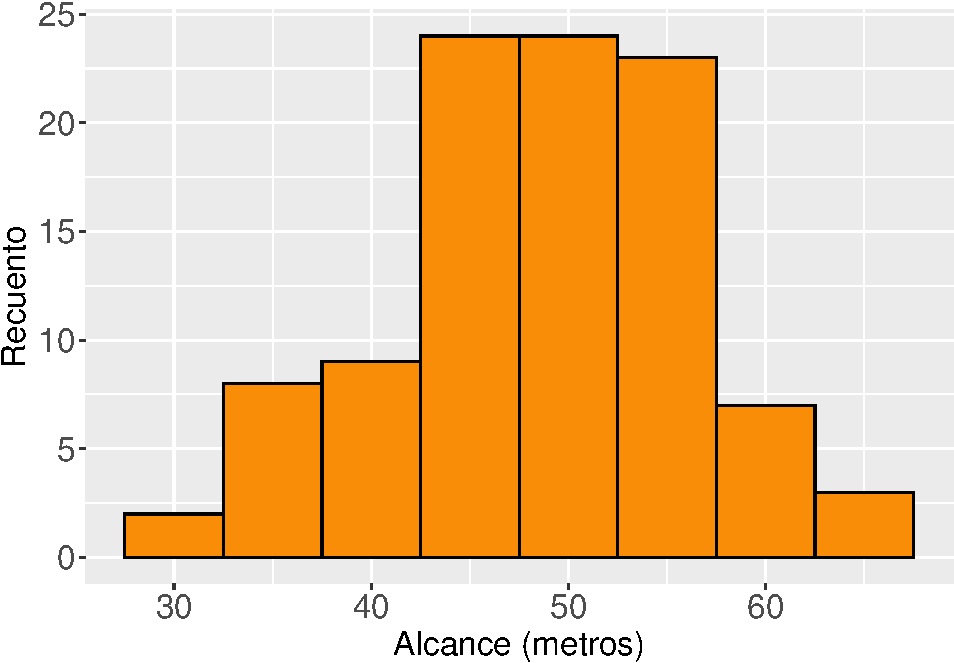
\includegraphics[width=0.8\linewidth]{one_mean_files/figure-latex/histog-1} \end{center}

\hypertarget{boxplot}{%
\subsection{Diagrama de caja y bigotes}\label{boxplot}}

Ahora vamos a representar las observaciones de la variable alcance mediante un gráfico que se denomina \textbf{diagrama de caja y bigotes}, usando la función \VERB|\FunctionTok{geom\_boxplot}\NormalTok{()}|:

\begin{Shaded}
\begin{Highlighting}[]
\FunctionTok{ggplot}\NormalTok{(}
  \AttributeTok{data =}\NormalTok{ mandos,}
  \AttributeTok{mapping =} \FunctionTok{aes}\NormalTok{(}
    \AttributeTok{x =} \StringTok{""}\NormalTok{,}
    \AttributeTok{y =}\NormalTok{ alcance}
\NormalTok{  )}
\NormalTok{) }\SpecialCharTok{+}
  \FunctionTok{geom\_boxplot}\NormalTok{()}
\end{Highlighting}
\end{Shaded}

\begin{center}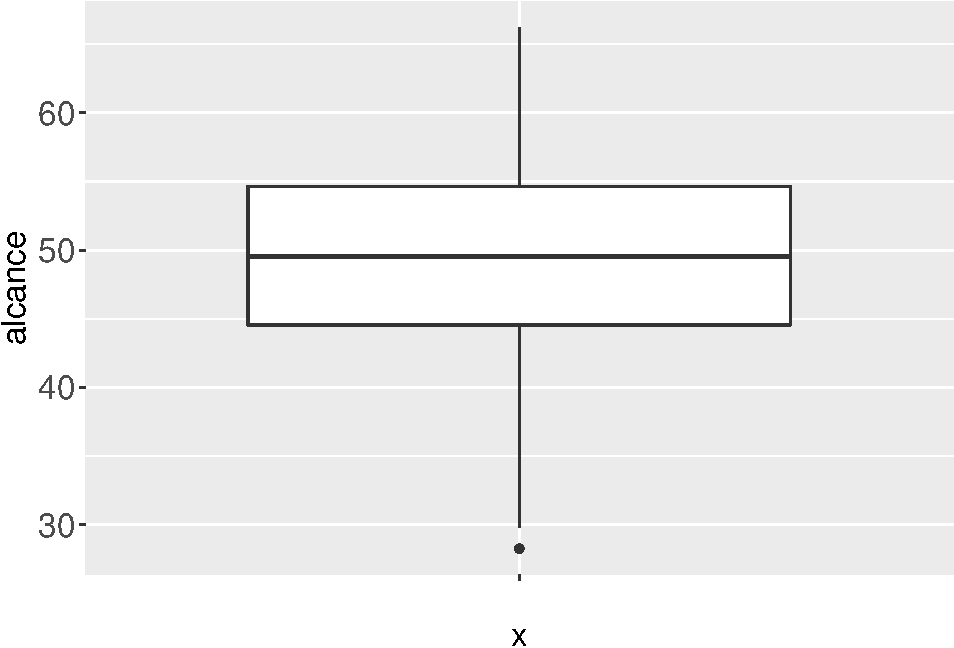
\includegraphics[width=0.8\linewidth]{one_mean_files/figure-latex/unnamed-chunk-26-1} \end{center}

Pasamos ahora a explicar cómo se construye e interpreta el diagrama de caja y bigotes que hemos dibujado.

\hypertarget{caja}{%
\subsubsection{Caja}\label{caja}}

La caja central del diagrama de caja y bigotes se construye con los valores de los cuartiles: la línea central se corresponde con la mediana y las líneas que delimitan la caja con el primer y tercer cuartil. De esta forma, la caja central contiene el \(50\%\) de los datos: el \(25\%\) en la mitad inferior de la caja, desde el primer cuartil hasta la mediana; y el \(25\%\) en la mitad superior, entre la mediana y el tercer cuartil.

\hypertarget{bigotes-y-outliers}{%
\subsubsection{Bigotes y outliers}\label{bigotes-y-outliers}}

Queda por explicar qué significan los \textbf{``bigotes''}, que son las líneas verticales por encima y debajo de la caja central, y por qué aparece resaltado un valor por debajo del bigote inferior.

El propósito de los bigotes es resaltar los datos extremos, muy pequeños, o muy grandes, que se denominan \textbf{outliers}. Datos por debajo del bigote inferior son catalogados como outliers por ser atípicamente pequeños, y datos por encima del bigote superior son considerados outliers por atípicamente grandes. Vemos que en nuestra muestra ha aparecido un oulier por debajo del bigote inferior, que, mirando la escala del eje \(Y\), vemos que tiene un valor menor que \(30\). Concretamente, se trata del valor mínimo \(28.26\) que apareció en primer lugar cuando ordenamos los datos de menor a mayor, y que podemos ver directamente calculando el mínimo:

\begin{Shaded}
\begin{Highlighting}[]
\FunctionTok{min}\NormalTok{(mandos}\SpecialCharTok{$}\NormalTok{alcance)}
\end{Highlighting}
\end{Shaded}

\begin{Shaded}
\begin{Highlighting}[]
\NormalTok{\#\# [1] 28.26}
\end{Highlighting}
\end{Shaded}

Los datos extremos u outliers pueden ser datos erróneos (debidos a errores en las mediciones, en la transcripción de los datos al fichero \(\dotsc\)). Pero también pueden ser datos correctos que, aun teniendo poca probabilidad de aparecer, han aparecido por azar en nuestra muestra. Aunque es una práctica frecuente desechar los outliers sistemáticamente, no es en absoluto una práctica recomendable. De hecho los outliers pueden ser lo más interesante de la muestra. La historia más famosa sobre las posibles consecuencias de la eliminación automática de outliers está relacionada con la detección del agujero de ozono. En 1985 se publicó el estudio mostrando que los niveles de ozono en la Antártida habían caído un \(10\%\) por debajo de lo normal. Se descubrió entonces que las mediciones inusualmente bajas del nivel de ozono ya habían sido registradas por el satélite Nimbus-7 de la NASA en 1976, pero que dichas mediciones fueron ignoradas al ser procesadas mediante un programa informático que descartaba automáticamente los valores excesivamente pequeños, como si se tratara de errores. De no ser por este tratamiento inadecuado de los outliers, el agujero de ozono podría haberse detectado casi una década antes.

Veamos cómo se dibujan los bigotes para decidir qué datos son outliers.
En primer lugar se calcula la diferencia entre tercer cuartil y primer cuartil (que es la anchura de la caja y se denomina \textbf{rango intercuartílico}) y se multiplica por \(1.5\). En nuestro caso, esta cantidad queda
\[
    1.5(54.66-44.545)=15.1725.
\]

Se catalogan como outliers aquellos valores que disten de los bordes de la caja central más de la cantidad anterior. En nuestro caso, serán outliers los valores inferiores a
\[
    44.545-15.1725=29.3725
\]
y los superiores a
\[
    54.66+15.1725=69.8325.
\]
El bigote inferior se extiende hasta el menor dato que no es considerado outlier. Y el bigote superior se extiende hasta el mayor dato que no es considerado outlier. Los datos por debajo y por arriba de los bigotes se clasifican como outliers.

Miremos de nuevo los primeros y últimos valores en la secuencia ordenada para nuestros \(100\) datos:

\begin{Shaded}
\begin{Highlighting}[]
\NormalTok{sorted }\OtherTok{\textless{}{-}} \FunctionTok{sort}\NormalTok{(mandos}\SpecialCharTok{$}\NormalTok{alcance)}
\FunctionTok{head}\NormalTok{(sorted)}
\FunctionTok{tail}\NormalTok{(sorted)}
\end{Highlighting}
\end{Shaded}

\begin{Shaded}
\begin{Highlighting}[]
\NormalTok{\#\# [1] 28.26 29.78 35.32 36.08 36.39 36.74}
\NormalTok{\#\# [1] 60.18 60.57 60.85 62.72 65.00 66.24}
\end{Highlighting}
\end{Shaded}

El único dato catalogado como outlier es \(28.26\), por eso el bigote izquierdo se extiende hasta \(29.78\) (el mínimo no outlier) y el bigote derecho hasta \(66.24\) (el máximo, no outlier).

\hypertarget{personalizaciuxf3n}{%
\subsubsection{Personalización}\label{personalizaciuxf3n}}

El siguiente código incluye varias opciones para personalizar el aspecto del diagrama de caja y bigotes creado al comienzo.

\begin{Shaded}
\begin{Highlighting}[]
\FunctionTok{ggplot}\NormalTok{(}
  \AttributeTok{data =}\NormalTok{ mandos,}
  \AttributeTok{mapping =} \FunctionTok{aes}\NormalTok{(}
    \AttributeTok{x =} \StringTok{""}\NormalTok{,}
    \AttributeTok{y =}\NormalTok{ alcance}
\NormalTok{  )}
\NormalTok{) }\SpecialCharTok{+}
  \FunctionTok{geom\_boxplot}\NormalTok{(}
    \AttributeTok{fill =} \StringTok{"\#08C9F9"}\NormalTok{,}
    \AttributeTok{outlier.colour =} \StringTok{"red"}\NormalTok{,}
    \AttributeTok{outlier.size =} \DecValTok{2}\NormalTok{,}
    \AttributeTok{outlier.shape =} \DecValTok{8}
\NormalTok{  ) }\SpecialCharTok{+}
  \FunctionTok{labs}\NormalTok{(}
    \AttributeTok{x =} \StringTok{""}\NormalTok{,}
    \AttributeTok{y =} \StringTok{"Alcance (metros)"}
\NormalTok{  ) }\SpecialCharTok{+}
  \FunctionTok{scale\_x\_discrete}\NormalTok{(}\AttributeTok{breaks =} \ConstantTok{NULL}\NormalTok{) }\SpecialCharTok{+}
  \FunctionTok{coord\_flip}\NormalTok{()}
\end{Highlighting}
\end{Shaded}

\begin{center}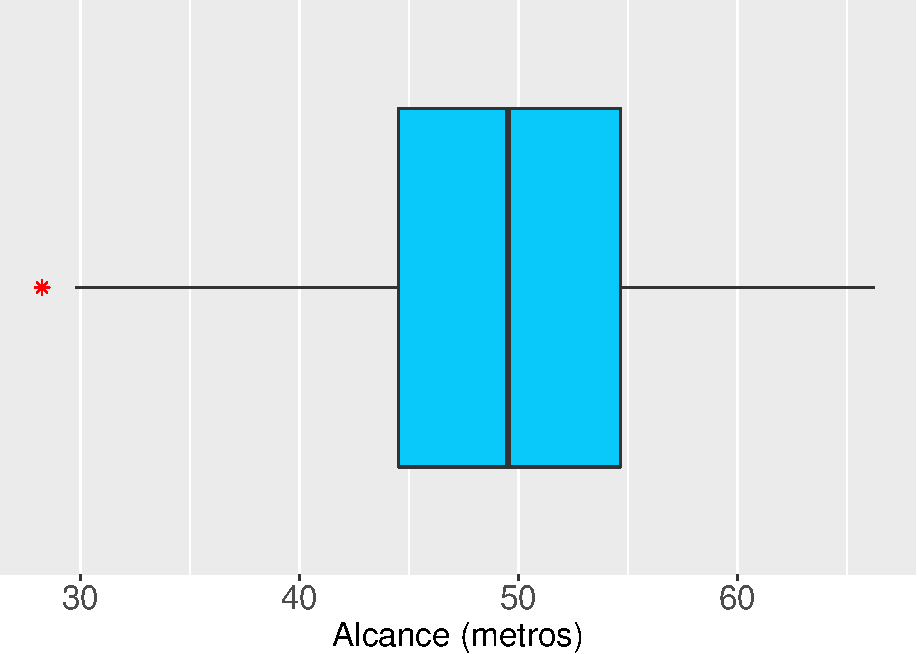
\includegraphics[width=0.8\linewidth]{one_mean_files/figure-latex/unnamed-chunk-29-1} \end{center}

\hypertarget{contraste-de-hipuxf3tesis}{%
\section{Contraste de hipótesis}\label{contraste-de-hipuxf3tesis}}

Hasta ahora hemos descrito los datos numérica y gráficamente.
Retomamos ahora el siguiente problema de inferencia estadística planteado al inicio:

\begin{ebox}{}
A nivel de significación \(0.05\) ¿puede afirmarse que los datos recogidos contradicen la afirmación de la empresa de que el radio de alcance medio de sus mandos es superior a \(50\) metros?

\end{ebox}

Según la empresa \(\mu>50\). Sin embargo, la estimación de la media poblacional \(\mu\) que proporcionan nuestros
datos es la media muestral
\[\overline{x}=48.8852,\] sugiriendo la hipótesis alternativa \(\mu < 50\). Planteamos en consecuencia el siguiente contraste de hipótesis para la media \(\mu\):

\[
  \left\{
    \begin{array}{lc}
    H_0:\ & \mu= 50\\
    H_1:\ & \mu <50
    \end{array}
    \right.
\]

Como ya sabemos, la hipótesis \(H_0\) se denomina hipótesis nula y la hipótesis \(H_1\) hipótesis alternativa.

Conocemos la función \VERB|\FunctionTok{binom.test}\NormalTok{()}| para calcular el \(p\)-valor asociado a un contraste de hipótesis para una proporción.
La función de \textsf{R} que usaremos ahora para resolver nuestro contraste de hipótesis sobre una media y calcular el \(p\)-valor asociado es \VERB|\FunctionTok{t.test}\NormalTok{()}|. Concretamente, tenemos que ejecutar el siguiente código:

\begin{Shaded}
\begin{Highlighting}[]
\FunctionTok{t.test}\NormalTok{(}
  \AttributeTok{x =}\NormalTok{ mandos}\SpecialCharTok{$}\NormalTok{alcance,}
  \AttributeTok{mu =} \DecValTok{50}\NormalTok{,}
  \AttributeTok{alternative =} \StringTok{"less"}
\NormalTok{)}
\end{Highlighting}
\end{Shaded}

\begin{Shaded}
\begin{Highlighting}[]
\NormalTok{\#\# }
\NormalTok{\#\#  One Sample t{-}test}
\NormalTok{\#\# }
\NormalTok{\#\# data:  mandos$alcance}
\NormalTok{\#\# t = {-}1.4757, df = 99, p{-}value = 0.07159}
\NormalTok{\#\# alternative hypothesis: true mean is less than 50}
\NormalTok{\#\# 95 percent confidence interval:}
\NormalTok{\#\#     {-}Inf 50.1395}
\NormalTok{\#\# sample estimates:}
\NormalTok{\#\# mean of x }
\NormalTok{\#\#   48.8852}
\end{Highlighting}
\end{Shaded}

En la salida anterior vemos que el \(p\)-valor de nuestro contraste es \(0.07\).

Recordemos que, en general, el \(p\)-valor de un contraste es la probabilidad de observar valores tan extraños como en la muestra si la hipótesis nula fuera cierta, entendiendo por valores extraños valores más a favor de la hipótesis alternativa que de la nula.
En este caso, el \(p\)-valor \(0.07\) se interpreta como la probabilidad de observar una media muestral tan pequeña como \(\overline{x}=48.89\) si \(H_0\) fuera cierta, es decir, si \(\mu=50\).

Recordemos también que el nivel de significación \(\alpha = 0.05\) fija el valor umbral con el que comparar el \(p\)-valor para tomar la decisión final en el contraste de hipótesis, de acuerdo con la siguiente regla:
Si el \(p\)-valor es inferior a \(0.05\) rechazamos la hipótesis nula en favor de la alternativa, concluyendo que los datos arrojan suficiente evidencia para afirmar que \(\mu<50\) y contradicen por tanto la afirmación de la empresa.
Si por el contrario el \(p\)-valor es superior a \(0.05\) no rechazamos la hipótesis nula, y decimos que no hay suficiente evidencia para contradecir la afirmación de la empresa.

Como en nuestro caso hemos obtenido un \(p\)-valor de \(0.07\), mayor que \(\alpha = 0.05\), no rechazamos la hipótesis nula, y concluimos que nuestros datos no proporcionan suficiente evidencia para contradecir la afirmación de la empresa. La ligera diferencia de la media muestral \(\bar{x} = 48.89\) respecto a \(50\) no ha resultado significativa para poder concluir que \(\mu<50\).

\hypertarget{conf_int}{%
\section{Intervalo de confianza}\label{conf_int}}

En la salida del comando \VERB|\FunctionTok{t.test}\NormalTok{()}| encontramos también el fragmento

\begin{center}{}

\begin{verbatim}
95 percent confidence interval:
    -Inf 50.1395
\end{verbatim}

\end{center}

´
que nos dice que un intervalo de confianza del \(95\%\) para la media \(\mu\) es:
\[(-\infty, 50.1395).\]

Como sabemos, un intervalo de confianza del \(95\%\) para un parámetro, incluye los valores del parámetro que no serían rechazados en un contraste de hipótesis a nivel de significación \(0.05\).

En este caso, el extremo derecho del intervalo de confianza obtenido, \(50.1395\), nos da el mayor valor aceptable para \(\mu\) a la vista de nuestro datos. Así, si bien no hemos encontrado suficiente evidencia en nuestros datos para afirmar, con un \(95\%\) de confianza, que \(\mu<50\), sí nos permitirían concluir que \(\mu<55\) (y que \(\mu\) es menor que cualquier valor superior a \(50.1395\)).

\printbibliography

% This file is created the first time epdf_document is invoked
% but will not be overwriten afterwards.
%
% After Body

\end{document}
